%! Author = mac
%! Date = 2022/4/1

\documentclass[UTF8]{ctexart}
\usepackage{geometry}
\geometry{left = 1.0cm, right = 1.0cm, top = 2.0cm, bottom = 2.0cm}
\usepackage{graphicx}
\usepackage{amssymb}



\title{关于 \LaTeX 的排版尝试}
\author{Q.D.}
\date{长春 \quad 朝阳 \quad 2022疫情期间}


\begin{document}

\maketitle

\section{序言}

\paragraph{序言}
此文档是对于本人学习使用 \LaTeX 的记录,
现在所记录的文字是 \kaishu{序言}。
\paragraph{编译器} 推荐使用XeLaTeX进行编译,否则会字体报错。


\subsection{基本格式}

\LaTeX \songti{存在}\heiti{多级标题},以及不同字体,
\kaishu{后文字体会继承最后一次声明(我也不知道是特性还是什么「笑」,这句没被继承是因为我再次声明了)。}
\paragraph{} 多级标题最多到$\backslash$subsubsection\{\},即1.1.1。
\paragraph{} 注意该节第一行,字体声明之间的空格会被识别,
比如这样(空格用"|"代替以直观演示):

\paragraph{} %增加一个空行
 $\backslash$LaTeX $\backslash$songti\{存在\} | $\backslash$heiti\{多级标题\}
\quad
会产生
\quad
\LaTeX \songti{存在} \heiti{多级标题}
\quad
\kaishu{的效果}。
\paragraph{} 推测为命令之间的空格都会被识别,且无论有几个底层空格都只识别一个,
多个空格可以通过$\backslash$quad命令实现,该命令后需要一个底层空格。
\paragraph{} 利用 $\backslash$backslash\$ 符号可以输出转义的$\backslash$ 符号,
\{\}直接用 $\backslash$ 转义即可,此类转义符号后的空格不被识别
\paragraph{} 本行利用"$\backslash$paragraph\{\}"命令另起一行,这几行都是。
并且命令后需要一个底层空格实现规范的段首对齐,建议其他命令后均附加一个底层空格。
\paragraph{} 本节首语进行以上细节的说明,以下是其他有关格式的内容。



\subsubsection{页间距}
\paragraph{}
页间距可以通过宏包geometry调整,利用"$\backslash$usepackage\{\}"命令
调用宏包。四个方向的边距分别用left、right、top、bottom表示。格式为direction = xcm。

\subsubsection{章节}
\paragraph{}
$\backslash$section{} 命令中,在\{\}前加入*可以使章节不编号

\subsubsection{段落}

\paragraph{段落}
正常段落用于正文的呈现。


\subparagraph{分段}
分段是段落的下一级,可用于长文本的引用。

\subsection{数学表达式}

\subsubsection{数学符号}
\paragraph{上下标} \LaTeX 存在对字符对上下标,比如$a^{2x+3}$与$a_{2}$,
 通过\$a\^{}\{2x+3\}\$以及\$a\_\{2\}\$实现。
\paragraph{分数} 形如分数$\frac{x}{3}$,可通过$\backslash$frac\{x\}\{3\}实现。
\paragraph{矢量} 对于矢量的表示方法则为 $\vec{a}$ 与 $\overrightarrow{xy}$,
 通过\$$\backslash$vec\{a\}\$与\$$\backslash$overrightarrow\{xy\}\$实现。
 \paragraph{括号} 对于括号见下表。

\begin{figure}[htbp]
\centering
\paragraph{} 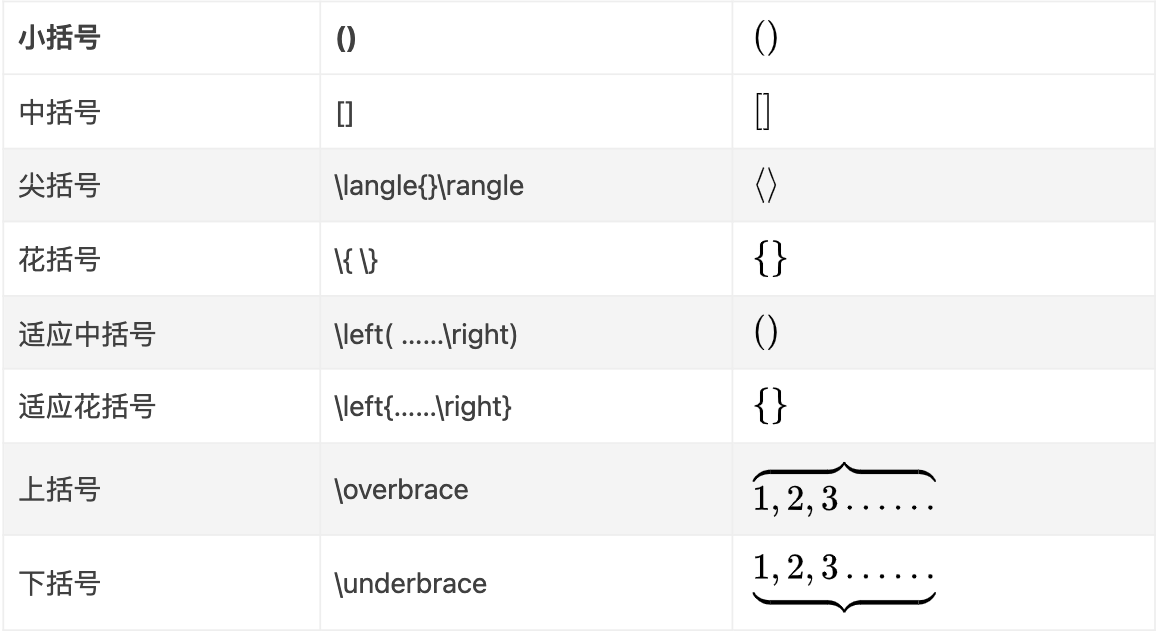
\includegraphics[height = 5.0cm]{/Users/mac/Desktop/ALLDATA/程序/TEX/学习过程/括号}\label{fig:figure}
\end{figure}

\paragraph{其他符号} 对于一些符号见下表。

\begin{figure}[htbp]
 \centering
 \paragraph{} 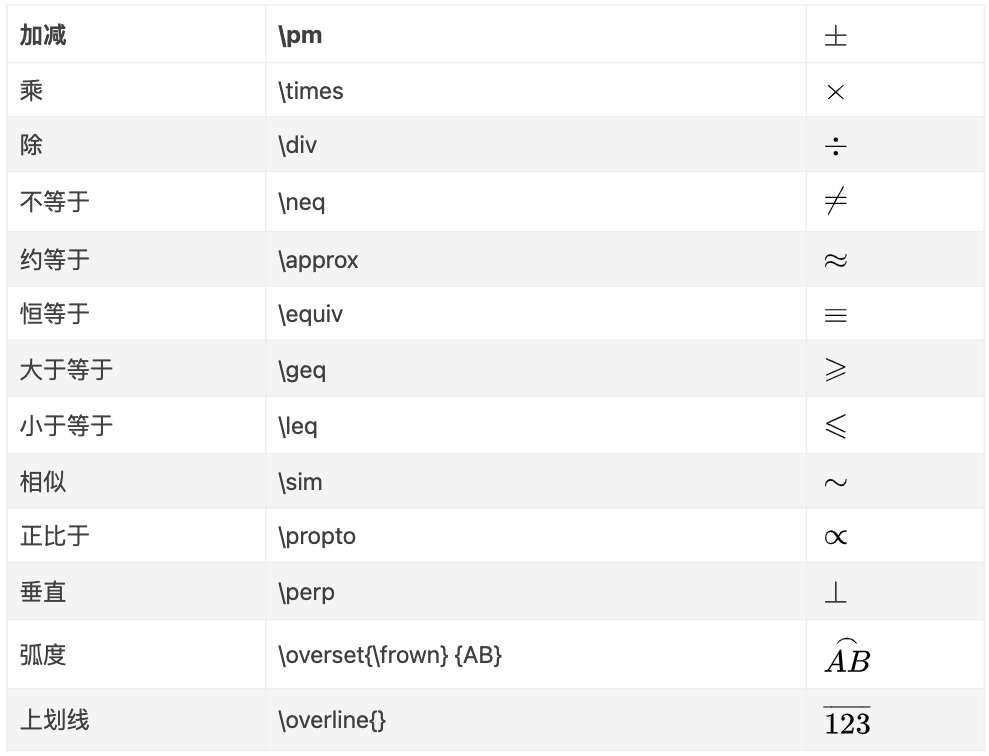
\includegraphics[height = 5.0cm]{/Users/mac/Desktop/ALLDATA/程序/TEX/学习过程/运算符号}\label{fig:figure2}
\end{figure}
\paragraph{比较类} $a \gg b$,$\pi \ll 10^{9}$,通过$\backslash$gg与$\backslash$ll实现。$c \textgreater d$,$\sqrt {2} \textless \sqrt {3}$,则通过
$\backslash$textgreater与$\backslash$textless实现

\paragraph{三角符号} 三角形符号$\Delta$,夹角 $\angle{}ABC$,角度 $30\,^{\circ}$,分度 $59'$。

 \paragraph{求和与累积} 求累加$\displaystyle\sum_{i = 1}^{n}x_i$,
求极限$\displaystyle\lim_{x \to +\infty}$,求累积$\displaystyle\prod_{i=1}^n x_i$,
求导数$x\prime$。



\paragraph{积分与微分} 对于微积分符号见下表。

\begin{figure}[htbp]
 \centering
 \paragraph{} 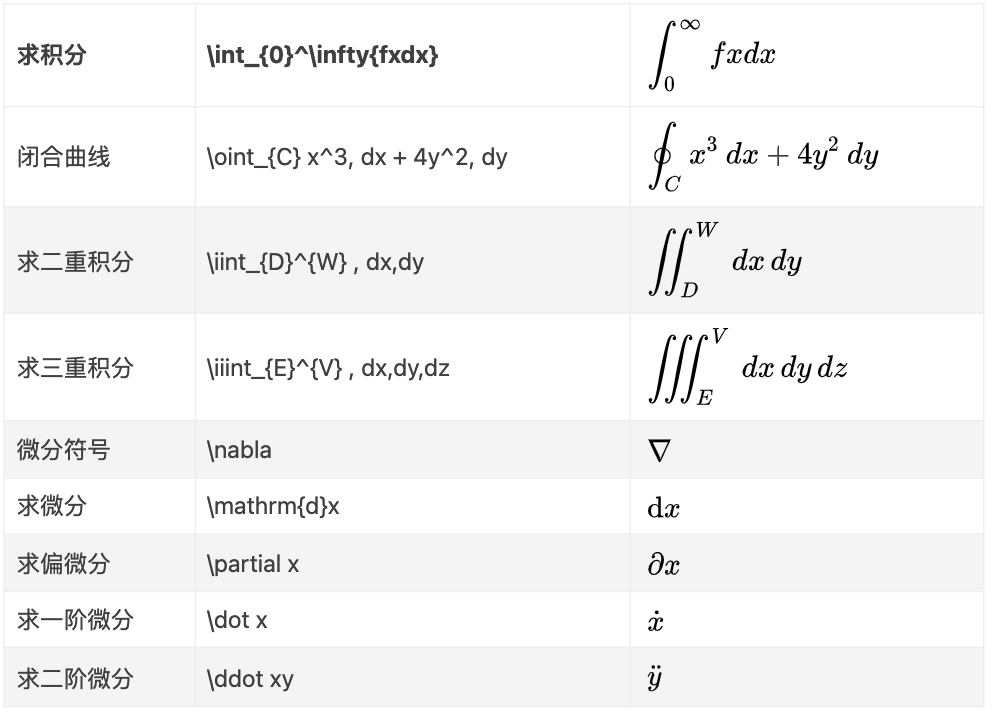
\includegraphics[height = 5.0cm]{/Users/mac/Desktop/ALLDATA/程序/TEX/学习过程/微积分}\label{fig:figure3}
\end{figure}

\paragraph{根号与分式} $\sqrt[3]{2x+3}$,$\frac {2^{x}+4x^{2}}{e^{2}}$

 \paragraph{集合} 对于集合符号见下表。

\begin{figure}[htbp]
 \centering
 \paragraph{} 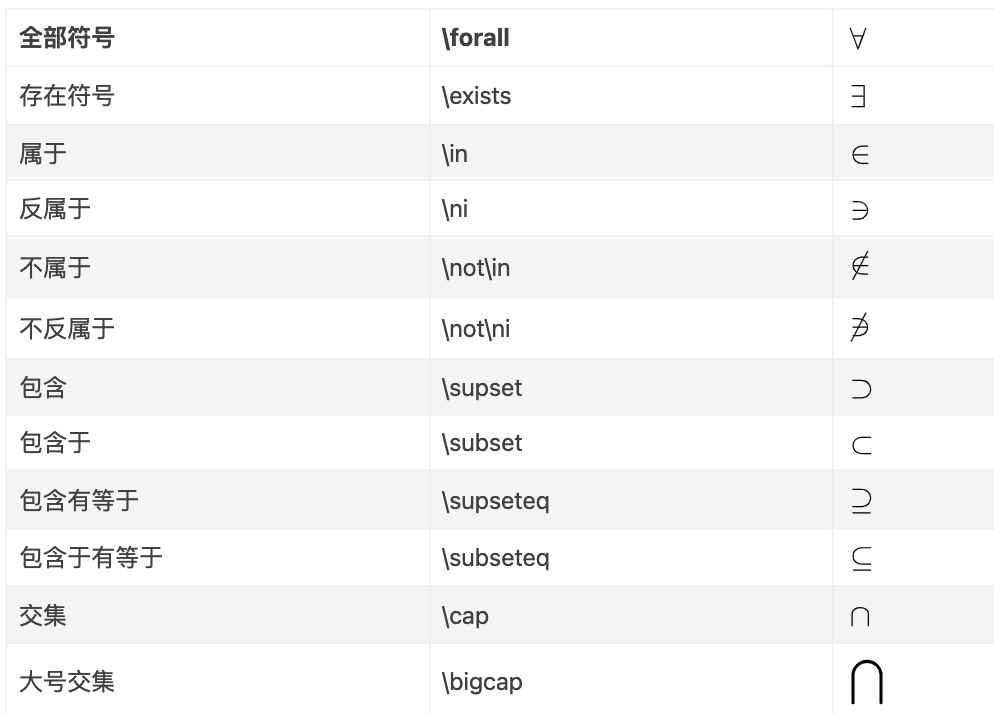
\includegraphics[height = 6.0cm]{/Users/mac/Desktop/ALLDATA/程序/TEX/学习过程/集合一}\label{fig:figure4}
 \paragraph{} 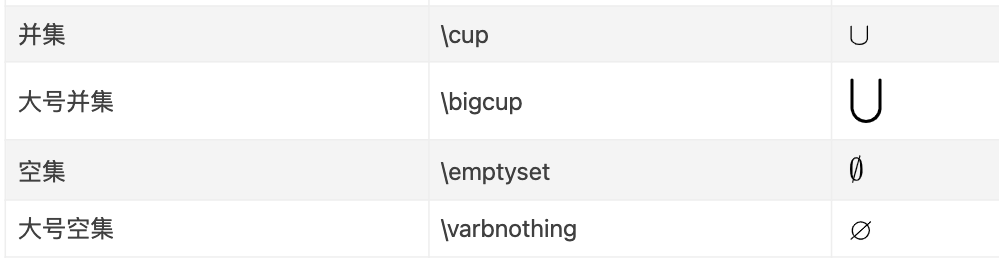
\includegraphics[height = 5.0cm]{/Users/mac/Desktop/ALLDATA/程序/TEX/学习过程/集合二}\label{fig:figure5}
\end{figure}


\end{document}